\chapter{Fazit}\label{cha:fazit}
Die ursprüngliche Frage dieser Arbeit war, wie genau wird das Ergebnis einer Elementarladung sein, wenn das Experiment, das vor über hundert Jahren entwickelt wurde, heute wiederholt wird. Die Antwort, verblüffend genau. Mithilfe eines Experimentierkasten wurde dieses Experiment durchgeführt und das Ergebnis war zuerst ernüchternd. Es musste vieles beachtet werden, unter anderem war das schwierigste die sorgfältige Berechnung der Ladung. Die Berechnung hängt von 12 verschiedenen Grössen ab, die alle verschiedene Einheiten haben und verschiedene Grössenordnungen. Wenn hier nicht konzentriert gearbeitet wurde, war das Ergebnis am Schluss falsch. Eine andere Hürde war das Messen. Wo genau waren jetzt diese 0.5mm Linien oder war genug Spannung vorhanden, wurde die Luftviskosität richtig abgelesen. All diese Sachen gaben am Anfang Probleme ein brauchbares Resultat zu bekommen. Mit der Zeit wurden diese Sachen behoben und man bekam auf einmal Ergebnisse, die in der Grössenordnung von $10^{-19}$ waren. Die Zuversicht stieg und man war verblüfft als man das Ergebnis in den Händen hatte. 

\section{Methoden}\label{sec:methoden}
Dieses Experiment verlangt viel Geduld und Nerven. Das Problem war das Ausrechnen. Man hat eine riesige Formel vor sich und ungefähr 40 verschiedene Messungen. Wie kann man den Prozess vereinfachen und somit Zeit effizient nutzen? Die Antwort liegt in der Programmierung. Für das Ausrechnen der Ergebnisse wurde Python verwendet. Mit dem Panda Modul können Daten von Excel-Tabellen gelesen, verarbeitet und wieder zurückgeschrieben werden \parencite{Inc_2024}. 

Da diese Arbeit in \LaTeX geschrieben wurde, mussten alle Grafiken von einem .png Format in ein .pdf Format umgeschrieben werden. Auch diese Sache übernahm ein Python skript. 

Im Allgemeinen wurden auch Programmierkenntnisse mit dieser Arbeit verbessert. Das Arbeiten mit \LaTeX war neu und schwierig am Anfang, hat sich aber gelohnt, durch die Vereinfachung von Formel schreiben und Formatierung einer wissenschaftlichen Arbeit. 

\section{Resümee}\label{sec:resumee}
Diese Arbeit hat aufgezeigt, wie es ist im Fach Physik ein fortgeschritteneres Experiment durchzuführen. Man lernte wie Messreihen aufgestellt werden, wie ein Experiment sorgfältig geplant werden muss oder dass nicht aufgegeben werden soll wenn nicht ein gewünschtes Ergebnis erscheint. Das Experiment wird nicht auf das erste Mal funktionieren. Es braucht Übung, Wissen und Planung, sonst wird das Experiment nicht gelingen. Es erfolgt zudem er Erwerb von Wissen, dass es nicht schadet sich Hilfe zu holen bei Fachpersonen und anderen Mitschüler. Das Experimentieren gelang erst als ein Assistenten dazugeholt wurde. \\

\noindent Die vorliegende Arbeit hat gezeigt, dass sich eine sorgfältige Arbeitsweise auszahlen kann und dass die Inanspruchnahme von externer Hilfe bei Schwierigkeiten zu einem erfolgreichen Ergebnis führen kann.

\begin{figure}[h]
	\centering
	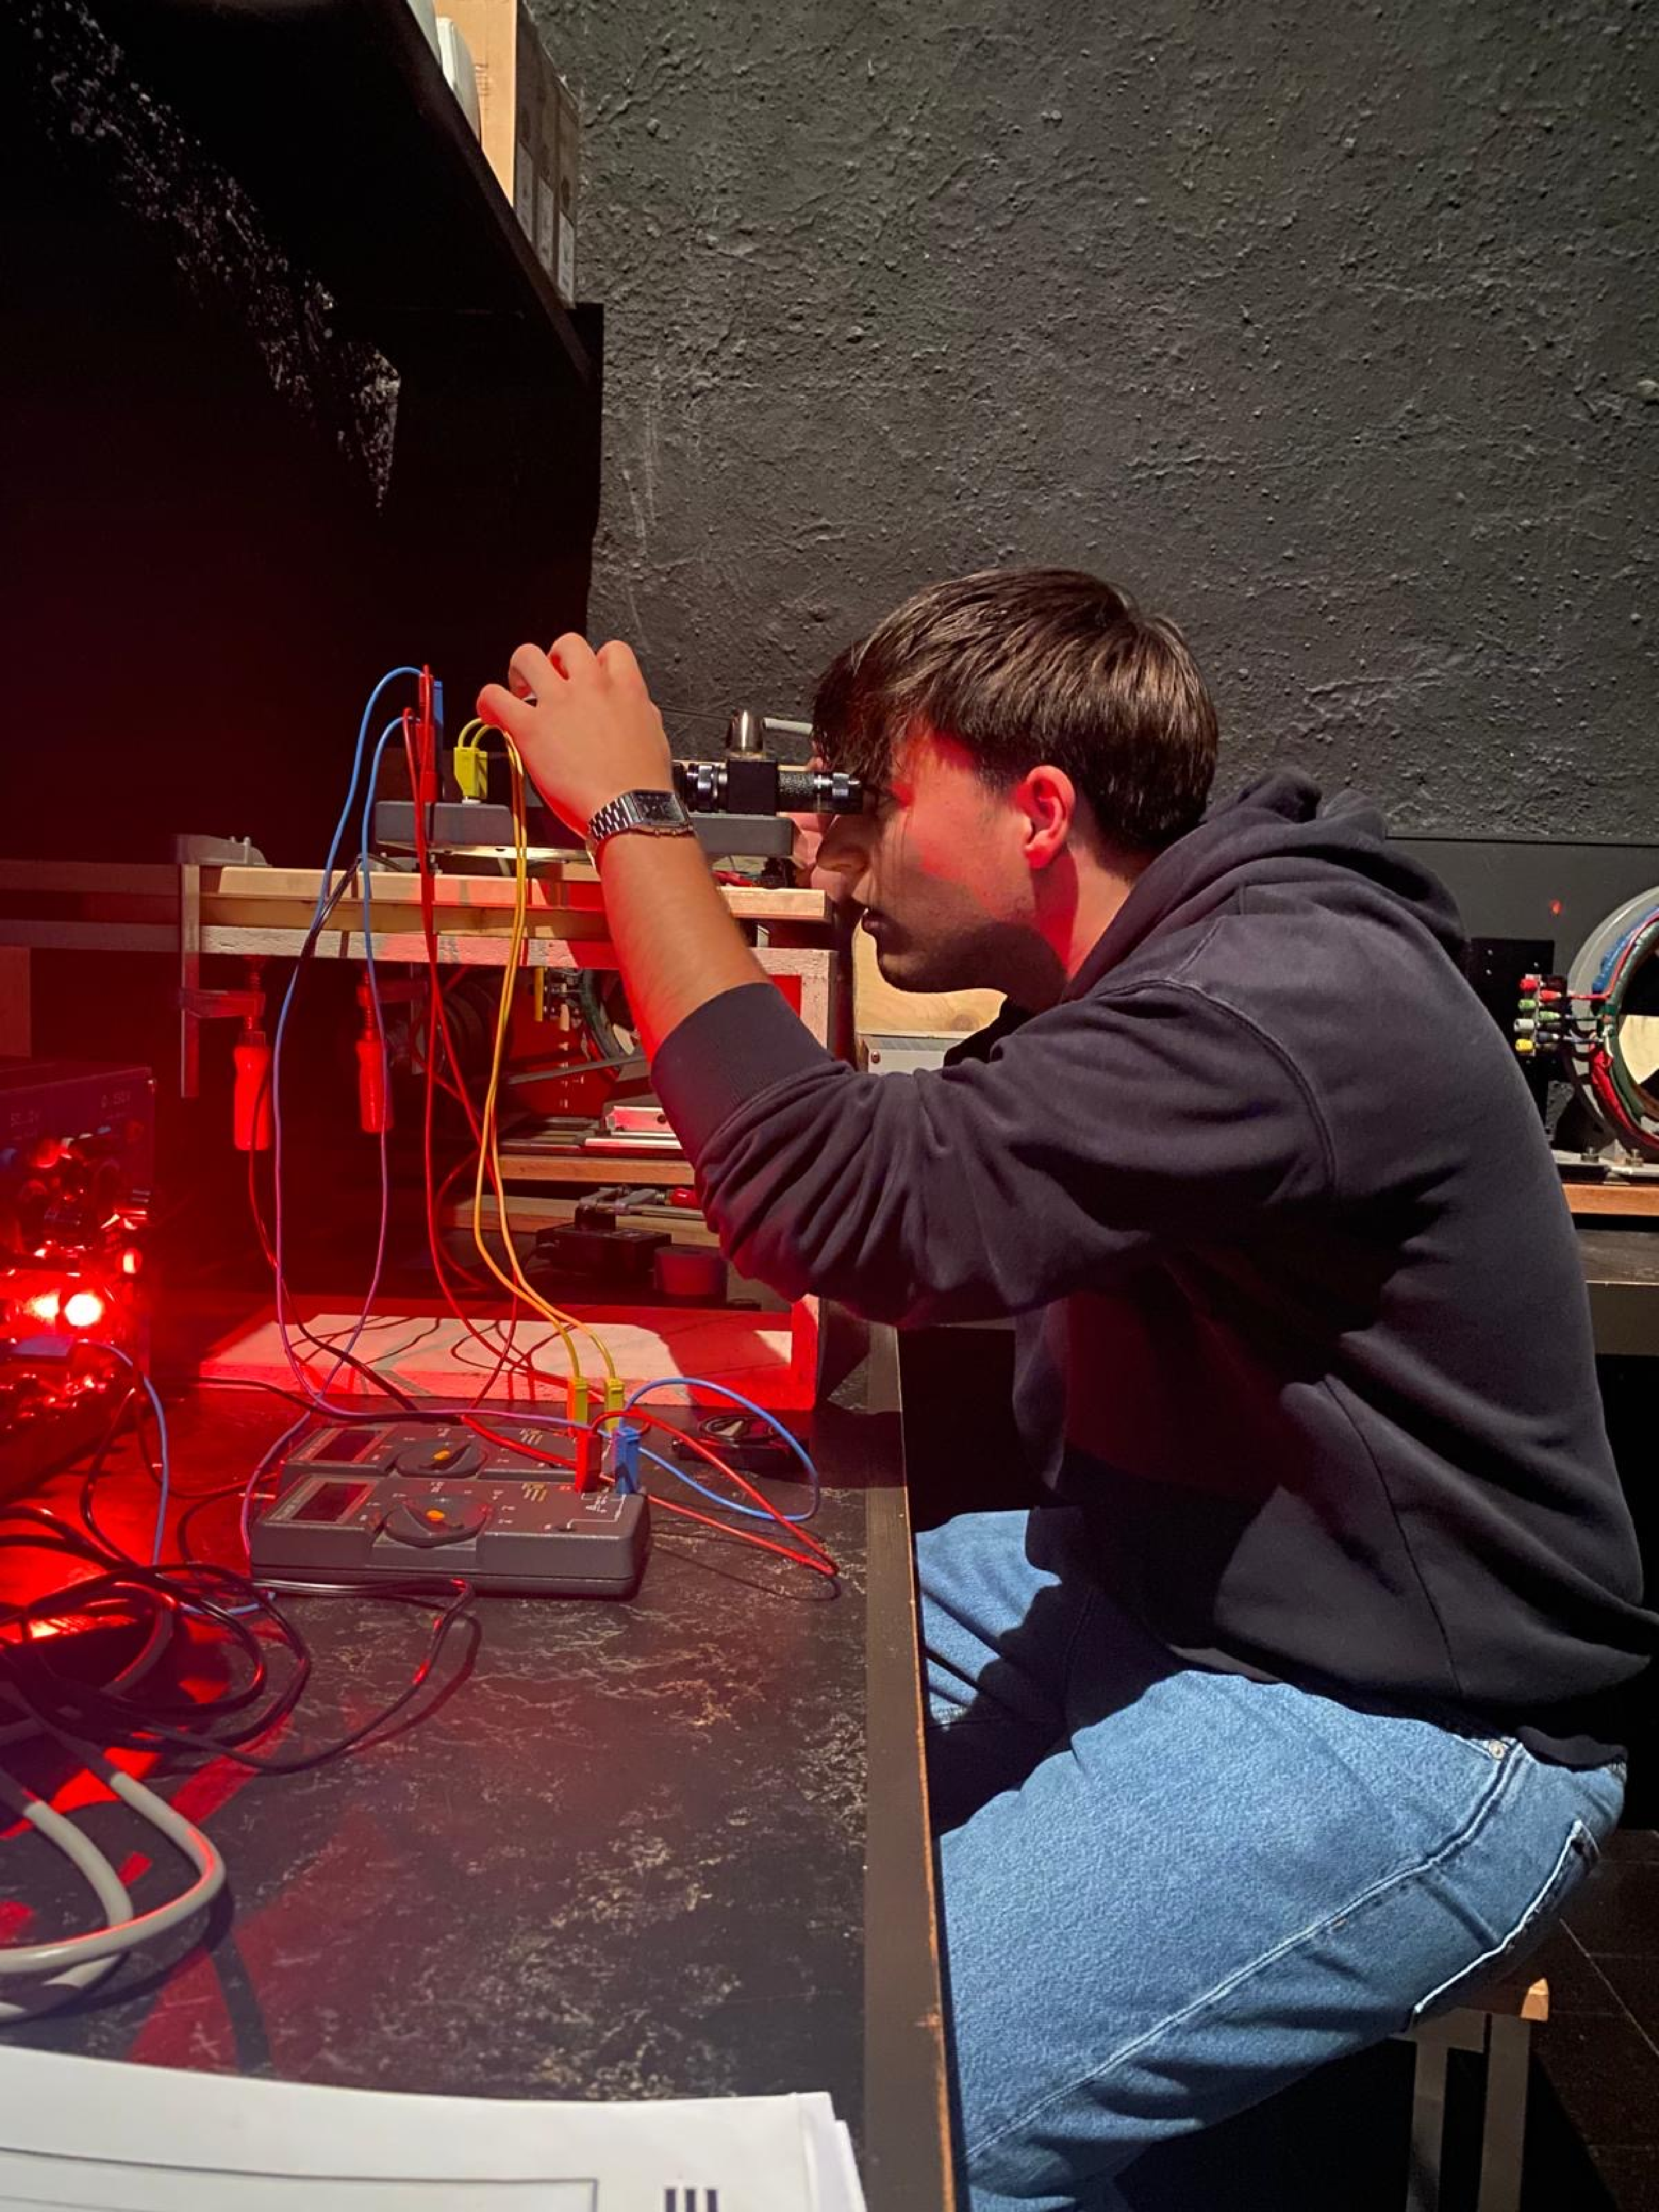
\includegraphics[scale=0.25]{bilder/pdf/bildExperimentieren.pdf}
	\caption{Bild während dem Experimentieren}
	\label{fig:experimentieren}
\end{figure}